%!TEX root = ../ausarbeitung.tex
\section{Aufteilung auf Sequenzen}

\subsection{Sortierung mithilfe der Exif-Daten}

Die handelsüblichen Kamerafallen haben einen Sensor, der bei Bewegung auslöst und zunächst zehn Bilder im Abstand von jeweils einer Sekunde schießt. Sollte es am Ende einer Zehnersequenz weiterhin Bewegung im Sichtfeld der Kamera geben, löst der Sensor erneut aus und es werden weitere zehn Bilder aufgenommen. Das sorgt dafür, dass der Datensatz aus zusammenhängenden Sequenzen von jeweils zehn oder mehr Bildern besteht. Oft befinden sich gerade auf den letzten Aufnahmen einer Sequenz keine Tiere mehr, da sich diese aus dem Bild bewegt haben. 

Unglücklicherweise sind die Daten auf der Datenbank lediglich nach Tierart sowie dort jeweils nach Tag und Nacht, leeren Bildern und Fehlklassifizierungen sortiert. Für das korrekte Funktionieren unserer Segmentierungstechnik PCA ist es aber nötig, dass die Daten in zusammenhängenden Sequenzen vorliegen. Aus diesem Grund benutzen wir die Exif-Metadaten, um die Daten aufzuteilen. Diese Exif-Daten umfassen Informationen über das Bild, wie beispielsweise die Abmessungen, das Aufnahmedatum, die Belichtungszeit, den ISO-Wert und das Kameramodell.

Unser Algorithmus sammelt zunächst die Metadaten aller aufzuteilenden Bilder in einer Liste. Diese Liste wird primär nach Seriennummer der Kamera und sekundär nach Aufnahmezeitpunkt sortiert. Sollte es zwischen zwei benachbarten Bildern in der Liste zu einem Wechsel der Seriennummer kommen, so wissen wir, dass eine neue Sequenz beginnt. Ebenso gilt das für zwei Bilder, die von derselben Kamera aufgenommen wurden, deren Aufnahmezeitpunkte sich jedoch um mehr als ein paar Sekunden unterscheiden. Diese beiden Situationen markieren den Wechsel einer Sequenz anhand der wir unterscheiden können, welche Bilder zusammenhängen.

Leider gehört die Seriennummer nicht zu den ursprünglichen Exif-Metadaten. Stattdessen wird sie in die sogenannten \emph{Maker Notes} geschrieben, einem freien Datenfeld, dass die Kamerahersteller für ihre Zwecke benutzen können. Aktuell gibt es keine Python-Bibliothek, die das Maker-Note-Feld auslesen kann. Aus diesem Grund waren wir gezwungen die Perl-Bibliothek \enquote{ExifTool} \cite{exif} zu benutzen und auf sie mit Hilfe einer Python-Schnittstelle zuzugreifen.

Zugegebenermaßen ist die Verwendung der Metadaten nicht der eleganteste Weg Sequenzen zu bestimmen. Sie hat aber - anders als das Auslesen und Abgleichen der Pixel aus der linken oberen Ecke des Bildes - den Vorteil unabhängig vom Kamerahersteller und -modell zu sein und ist sehr effizient.

\begin{figure}
	\centering
	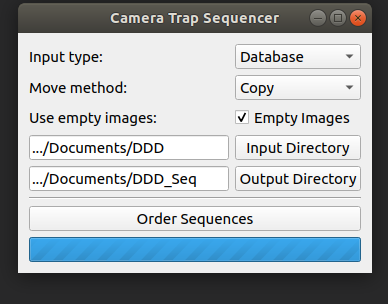
\includegraphics[scale=0.5]{img/CameraTrapSequencer.png}
	\caption{Der Camera Trap Sequencer im Linux-Design.}
\end{figure}

\subsection{Camera Trap Sequencer}

Der Camera Trap Sequencer ermöglicht es dem Anwender seine Datenbank mit Kamerafallenbildern unkompliziert und schnell auf Sequenzen aufzuteilen. Als Eingabe kann sowohl eine komplette Datenbank als auch ein einzelner Ordner mit Bildern benutzt werden. Man kann sich zwischen dem Verschieben und Kopieren der Bilder entscheiden. Das Verschieben von Bildern hat den Vorteil, dass keine Daten dupliziert werden. Die ursprüngliche Ordnerstruktur bleibt momentan jedoch noch erhalten. 

Abschließend hat man im Fall einer Bilddatenbank die Möglichkeit sich dafür zu entscheiden mit Informationen über leere Bilder zu speichern. Alle vorsortierten Datenbanken haben Verzeichnisse mit dem Namen \enquote{empty}, in denen sich Bilder auf Sequenzen befinden, auf denen keine Tiere zu sehen sind. Unsere Segmentierungstechnik PCA ist darauf angewiesen möglichst auf möglichst langen Bildsequenzen angewendet zu werden. Deshalb ist es nützlich, False-Positives mitzuverwenden, insbesondere weil leere Bilder einen großen Beitrag zur Berechnung eines leeren Hintergrundbilds leisten können. Da wir als Label für die Klassifizierung aber die Namen der Tierordner benutzen, müssen diese vor der Klassifizierung aussortiert werden. Deshalb speichern wir, falls die empty-Option gesetzt ist, eine Textdatei mit den Dateipfaden aller leeren Bilder, die dann im Anschluss an PCA aussortiert werden können. \\
Der Camera Trap Sequencer selbst ist mit PyQt5 umgesetzt. Er zeichnet sich deshalb durch ein natives Design auf jeder Plattform aus.
